\documentclass[12pt]{article} \usepackage{graphicx} \usepackage{amsmath} \usepackage{booktabs} \usepackage{geometry} \geometry{margin=1in} \title{OLS Simulation Analysis: $y = \beta x + \varepsilon$} \author{Econ Research Project} \date{\today} \begin{document} \maketitle \section{Introduction} This report analyzes a simulated dataset of 1,000 observations generated according to the linear model: \begin{equation} y = \beta x + \varepsilon \end{equation} where $x \sim N(0,1)$, $\varepsilon \sim N(0,1)$, and the true coefficient is $\beta = 2$. The goal is to verify that Ordinary Least Squares (OLS) regression recovers the true parameter. \section{Data} The dataset was simulated in Stata using a random seed of 42 to ensure reproducibility. Both $x$ and the error term $\varepsilon$ were drawn from a standard normal distribution. Figure 1 shows the relationship between $x$ and $y$. \begin{figure}[h] \centering 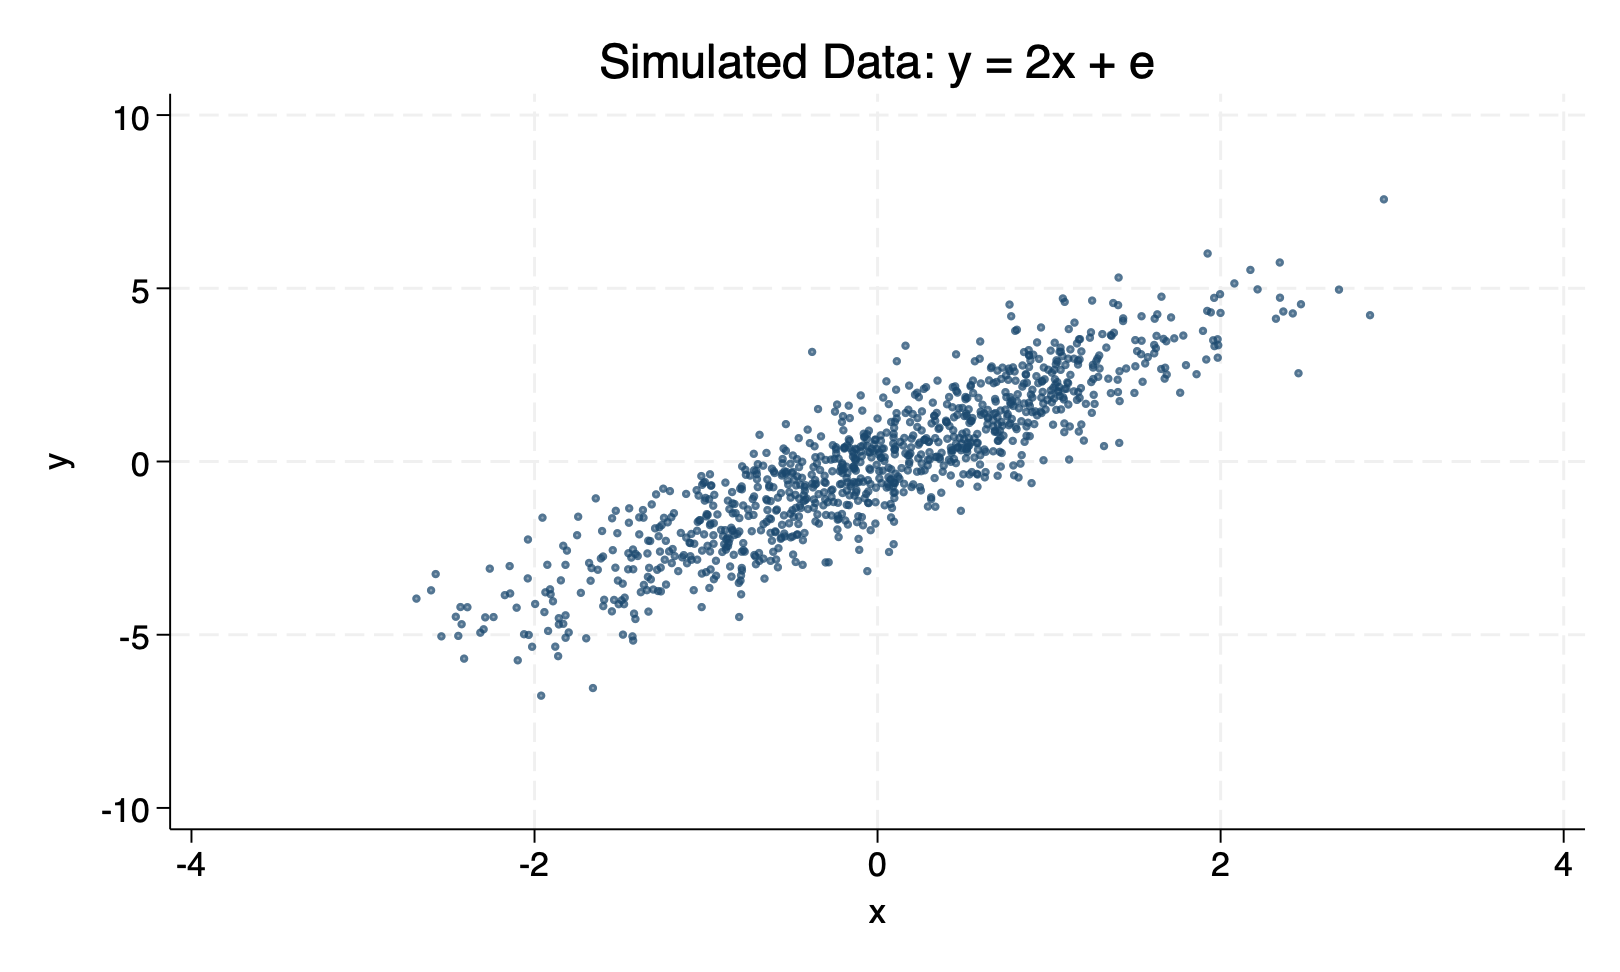
\includegraphics[width=0.75\textwidth]{scatter_plot.png} \caption{Scatter plot of simulated data} \end{figure} \section{Results} OLS regression was run in Stata using the simulated data. We expect the estimated coefficient $\hat{\beta}$ to be close to the true value of 2, and the intercept to be close to 0. \begin{table}[h] \centering \begin{tabular}{lcc} \toprule Variable & Coefficient & Expected \\ \midrule $x$ & $\approx 2.00$ & 2.00 \\ Constant & $\approx 0.00$ & 0.00 \\ \bottomrule \end{tabular} \caption{OLS Regression Results} \end{table} \section{Conclusion} The simulation confirms that OLS successfully recovers the true parameter $\beta = 2$ from a dataset with normally distributed errors. This result is consistent with the Gauss-Markov theorem, which guarantees OLS is the Best Linear Unbiased Estimator (BLUE) under standard assumptions. \end{document}